\documentclass{standalone}
\usepackage{tikz}
\usetikzlibrary{decorations.markings,
decorations.pathmorphing,
arrows,
positioning,
calc,
patterns}
\usepackage{pgfplots}
\usepackage{helvet}
\usepackage[eulergreek]{sansmath}
\pgfplotsset{compat=1.18}
\pgfplotsset{
    tick label style={font=\sansmath\sffamily},
    every axis label/.append style={font=\sffamily},
    legend style={font=\sffamily},
    title style={font=\sffamily}
}

\begin{document}

\definecolor{myRed}{RGB}{204,0,0}
\definecolor{myBlue}{RGB}{0,102,204}

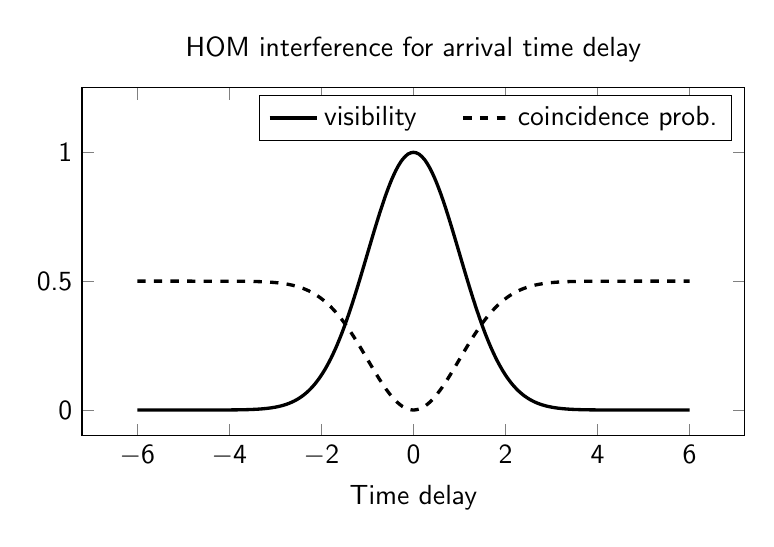
\begin{tikzpicture}

  \begin{scope}
  \begin{axis}[
    height=6cm,
    width=10cm,
    domain=-6:6,
    samples=101,
    ymin=-0.1,
    ymax=1.25,
    xlabel={Time delay},
    title={HOM interference for arrival time delay},
    legend entries={visibility,coincidence prob.},
    legend columns=2,
    legend style={/tikz/every even column/.append style={column sep=0.5cm}}]

  \addplot [black, very thick, smooth] {exp(-0.5*x*x)};
  \addplot [black, very thick, smooth, dashed] {0.5*(1-exp(-x*x/2))};

  \end{axis}
  \end{scope}

\end{tikzpicture}

\end{document}
